\documentclass[letterpaper]{article}
\usepackage{aaai}
\usepackage{hyperref}
\usepackage{lmodern}
\usepackage{courier}
\usepackage{listings}
\usepackage{graphicx}
\graphicspath{ {figures/} }
\usepackage[round]{natbib}

\lstset{basicstyle=\ttfamily\footnotesize,breaklines=true}

\setlength{\pdfpagewidth}{8.5in}
\setlength{\pdfpageheight}{11in}
\pdfinfo{
  /Title (Topic Modeling for Scientific Documents)
  /Author (Jethro Kuan)}
\begin{document}
\nocopyright
\bibliographystyle{plainnat}

\title{Topic Modeling for Scientific Documents}
\author{Jethro Kuan \\
  WING-NUS\\
}
\maketitle
\begin{abstract}
  \begin{quote}
    Topic models are statistical models, used to discover abstract
    topics that occur in a collection of documents. In this paper, we
    focus on the technique of topic modeling, particularly in its
    application to the domain of scientific documents. We discuss
    different approaches to topic modeling, and weigh in on their
    strengths and shortcomings.
  \end{quote}
\end{abstract}

\section{Introduction}
In this information age, the availability of knowledge is
insufficiently met with the tools to navigate it. Tools like Semantic
Scholar use machine learning to process scientific documents and
extract meaningful structure, empowering researchers to discover
papers more relevant to their work. One such technique is topic
modeling.

\section {Topic Modeling}
Topic Modeling attempts to discover abstract topics within documents.
Most topic models are generative models, assuming that latent
variables govern the generative process of a document.

For example, a topic model trained on a corpora of scientific
documents could learn topics such as ``Neural Networks'', ``Biology''
and ``Medicine''. Topics attribute a high probability to words that
relate to the topic. For example, a ``Neural Networks'' topic
would give attribute a high probability to ``classifiers'', and a low
probability to ``bacteria''. The quotations around the topics indicate
that the labels are human interpretations of what these topics may be.
Automatic labeling of these topics are also areas of research.
**CITE**

\begin{figure}[ht]
  \centering
  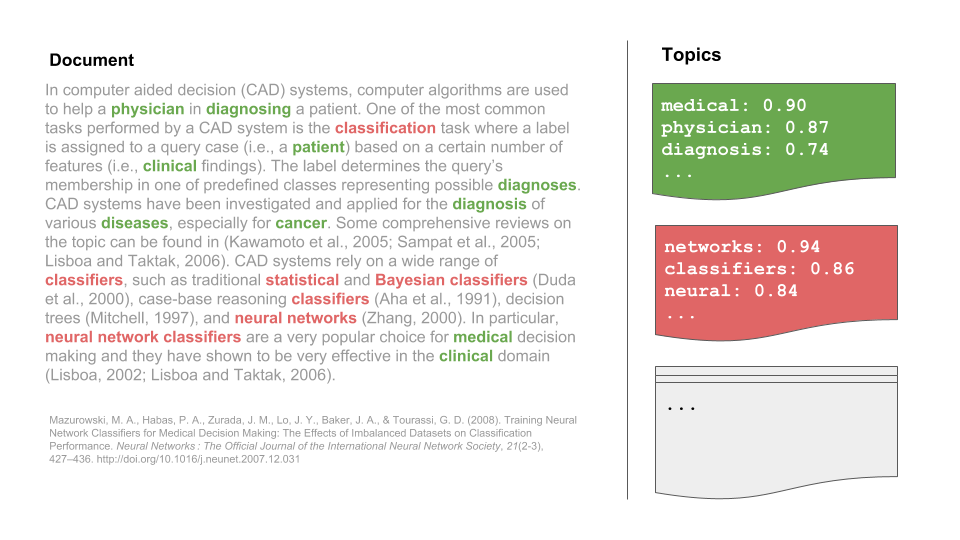
\includegraphics[width=0.5\textwidth]{topic_models.png}
  \caption{\label{fig:topic_model_document} According to the trained
    topic model, topics like ``Medicine'' and ``Neural Networks''
    generate the colored words of the document}
\end{figure}


Topic modeling may discover that document in
~\autoref{fig:topic_model_document} relates to ``Medicine'' and
``Neural Networks'', because these topics give rise to the colored
words in the document.

In addition, we can view these abstract topics as a form of clustering.
Researchers are better able to navigate the large corpora of
scientific knowledge, by exploring documents that have similar topic
proportions.

In this paper, we briefly discuss the predominant model: Latent
Dirichlet Allocation (LDA) and its variants. In addition, we explore
other models that are not derivatives of LDA, such as the Replicated
Softmax.

\section{LDA}
Latent Dirichlet analysis is widely considered to be the simplest
topic model. LDA models each document as a mixture of topics, where a
topic $\beta_k$ is a probability distribution over a fixed vocabulary
of terms.

The Dirichlet distribution encourages sparsity, encoding the belief
that the document-topic distribution has few topics per document, and
the topic-word distribution has few words per topic. These two beliefs
work against each other, and LDA discovers this sparsity balance,
which gives rise to the structure of the textual data.

The generative process of a document is as follows:

\begin{lstlisting}[mathescape=true]
for each document $w$ do
  Draw topic distribution $\theta \sim Dir(\alpha)$;
  for each word at position $n$ do
    Sample topic $z_n \sim Multinomial(\theta)$
    Sample word $w_n \sim Multinomial(\beta_{z_n})$
\end{lstlisting}

We can compute the probability of a word, given the LDA parameters:

\begin{equation}
  p(w | \alpha, \beta) = \int_\theta \left( \sum_{n=1}^{N}
    \sum_{z_n = 1}^{k} p(w_n | z_n, \beta)p(z_n | \theta) \right)
  p(\theta | \alpha) d\theta
\end{equation}

Posterior inference over the hidden variables $\theta$ and $z$ is
intractable due to the coupling between $\theta$ and $\beta$ under the
multinomial assumption. \citep{blei2003latent}. Hence, we rely on
techniques for approximate inference of the posterior. We discuss these
techniques in ~\autoref{sec:inference}.

\subsection{Statistical Assumptions}
\label{subsec:statistical-assumptions}
As Mackay quips, we cannot make inference without statistical
assumptions. LDA makes several assumptions, some rendering it less
suited for application to the domain of scientific documents.

1. The order of documents do not matter.

The meaning of keyphrases used in scientific literature change over
time. For example, neural networks meant a different thing two decades
ago.

2. Bag of Words

Variants of LDA relax these statistical assumptions, or make other
assumptions in place. We discuss Dynamic Topic Modeling (DTM) in
~\autoref{sec:dtm}, and briefly mention the rest in the appendix.

\section{Inference Methods}
\label{sec:inference}
Approximating intractable probability densities is a well-studied
problem in modern statistics. This problem arises often in Bayesian
statistics, where computing posterior probablity densities in requires
inference over latent variables. Many learning algorithms have been
developed, including collapsed Gibbs Sampling, Variational Inference,
Collapsed Variational Inference, and MAP estimation. Each of these
approximation techniques have their own strength and shortcomings.

The two inference methods are briefly discussed below, and a
comparison between them relegated to the appendix in
~\autoref{sub:choosing-inference}.

\subsection{MCMC Sampling}
\label{subsec:mcmc-sampling}
Historically, Markov Chain Monte Carlo (MCMC) sampling has been the
dominant technique for approximating posterior densities. In MCMC, we
construct an ergodic Markov chain on the latent variable $z$,
whose stationary distribution is the posterior $P( z | x)$.
Samples are drawn from the stationary distribution, and used to
approximate the posterior empirically.

\subsection{Variational Inference}
\label{subsec:vi}
Mean field variational inference (MFVI) breaks the coupling between
$\theta$ and $z$ by introducing free variational parameters $\gamma$
over $\theta$ and $\phi$ over $z$ and dropping the edges between them.
This results in an approximate posterior $q(\theta, z | \gamma, \phi)
= q_\gamma(\theta)\prod_nq_\phi(z_n)$.

To best approximate the true posterior, we frame it as an optimization
problem, minimizing $L$ where:

\begin{equation}
L(\gamma, \phi | \alpha, \beta) = D_{KL}\left[ q(\theta, z | \gamma,
  \phi) || p(\theta, z | \alpha, \beta) \right] - \log p(w | \alpha, \beta)
\end{equation}

This optimization has closed form coordinate descent equations for
LDA, because the Dirichlet is conjugate to the Multinomial
distribution. This computational convenience comes at the expense of
robustness, making it difficult to apply to other more complicated
topic models.

\section{Dynamic Topic Modeling}
\label{sec:dtm}
Dynamic Topic Modeling (DTM) was proposed to remove the assumption
that documents are \textit{exchangeable}. \citep{blei2006dynamic}

The order of documents are important for scientific documents, since
both the content, and the meaning of words evolve over time.

In DTM, data is divided by discrete time slices. The topics associated
with time slice $t$ evolve from the time slice $t-1$. Because the
Dirichlet distribution is not amenable to sequential modeling, we use
the Gaussian distribution to model the sequence of random variables.

The generative process for time slice $t$ is as follows:

\begin{lstlisting}[mathescape=true]
Draw topic distribution $\beta_t | \beta_{t-1} \sim N(\beta_{t-1},
  \sigma^2I)$;
Draw $\alpha_t | \alpha_{t-1} \sim N\left( \alpha_{t-1}, \delta^2I
  \right)$
for each document $w$ do
  Draw $\eta_{w,t} \sim N\left( \alpha_t, a^2I \right)$
  for each word at position $n$ do:
    Sample topic $z_{t,n} \sim Multinomial(\pi(\eta_{w,t}))$
    Sample word $w_{t,d,n} \sim Multinomial(\beta_{t,z,n})$
\end{lstlisting}

$\pi$ maps the multinomial parameters to the mean parameters,
$\pi\left( \beta_{k,t} \right)_w = \frac{exp(\beta_{k,t,w})}{\sum_w exp\left( \beta_{k,t,w} \right)}$

The Multinomial and Guassian distributions are not conjugates,
inference via Gibb's sampling is difficult. Hence, variational
inference instead.

Further extensions of this approach include the continuous Dynamic
Topic Models (cDTM), which removes the discretization of the time
slices. \citep{wang-2012-contin-time} This model has been used to
predict the timestamp of documents.

\section{Appendix}
\subsection{Choosing an Inference Method}
\label{sub:choosing-inference}
How do we know which technique to use to approximate the posterior
density? MCMC methods are computationally more intensive, but provide
samples that are approximately exact from the target posterior
density. In contrast, VI methods view the problem as an optimization
problem, which allows it to utilize efficient learning algorithms such
as stochastic optimization. This is much quicker to compute, and is
suited for larger datasets.

MCMC methods, however, cover a large family of sampling methods.
Gibb's sampling requires that the prior and posterior are conjugate
distributions. When this is not possible, such as in DTM, VI methods
can perform better than other methods in the MCMC family.

A closer look at the different inference approximation algorithms,
however, shows that the performance differences can be explained away
by setting certain smoothing hyperparameters
\citep{asuncion-2012-smoot-infer}.

\subsection{Alternatives to LDA}

\bibliography{survey}
\end{document}
